\documentclass[11pt, twoside, openright]{memoir}

% ── Core packages ─────────────────────────────────────────────────────────────
\usepackage{amsmath, amssymb, bm}
\usepackage{mathtools}
\usepackage[T1]{fontenc}
\usepackage[utf8]{inputenc}
\usepackage{palatino}
\usepackage{mathpazo}
\usepackage{microtype}

% ── Page geometry ─────────────────────────────────────────────────────────────
\usepackage[
  paperwidth=7in, paperheight=10in,
  top=1in, bottom=1in,
  inner=0.85in, outer=0.75in,
  includeheadfoot
]{geometry}

% ── Graphics, tables, color ───────────────────────────────────────────────────
\usepackage{graphicx}
\usepackage{booktabs}
\usepackage{array}
\usepackage{tabularx}
\usepackage[table]{xcolor}
\usepackage[most]{tcolorbox}
\usepackage{tikz}
\usetikzlibrary{arrows.meta, calc, positioning, decorations.pathreplacing}
\usepackage{listings}

% ── Lists, floats ─────────────────────────────────────────────────────────────
\usepackage{enumitem}
\usepackage{parskip}
\usepackage{float}
\usepackage{caption}
\captionsetup{font=small, labelfont=bf}

% ── References ────────────────────────────────────────────────────────────────
\usepackage{hyperref}
\hypersetup{colorlinks=true, linkcolor=Navy, urlcolor=Blue, citecolor=Teal,
  pdftitle={Layer-Time Geometry: How Language Models Process Information},
  pdfauthor={Agus Sudjianto and Aijun Zhang}}

% ── Colors ────────────────────────────────────────────────────────────────────
\definecolor{Navy}{HTML}{1F3864}
\definecolor{Blue}{HTML}{2E6DAD}
\definecolor{LBlue}{HTML}{DDEAF7}
\definecolor{Teal}{HTML}{1D6A6A}
\definecolor{LTeal}{HTML}{D6EFEF}
\definecolor{Amber}{HTML}{7B4A00}
\definecolor{LAmber}{HTML}{FFF3CD}
\definecolor{DGreen}{HTML}{1B5E20}
\definecolor{LGreen}{HTML}{E8F5E9}
\definecolor{DRed}{HTML}{7B1515}
\definecolor{LRed}{HTML}{FDECEA}
\definecolor{LGray}{HTML}{F5F5F5}
\definecolor{MGray}{HTML}{DDDDDD}
\definecolor{DGray}{HTML}{444444}
\definecolor{CodeBG}{HTML}{F7F7F7}

% ── Memoir styles ─────────────────────────────────────────────────────────────
\chapterstyle{veelo}
\renewcommand{\partnamefont}{\huge\sffamily\color{Navy}}
\renewcommand{\partnumfont}{\huge\sffamily\color{Navy}}
\renewcommand{\parttitlefont}{\Huge\bfseries\sffamily\color{Navy}}
\setsecheadstyle{\large\bfseries\sffamily\color{Navy}}
\setsubsecheadstyle{\normalsize\bfseries\sffamily\color{Blue}}
\setsubsubsecheadstyle{\normalsize\bfseries\itshape\color{Teal}}
\pagestyle{ruled}

% ── tcolorbox environments ─────────────────────────────────────────────────────
\tcbset{
  base/.style={enhanced, breakable, left=6pt, right=6pt, top=6pt, bottom=6pt,
    fontupper=\small, before upper={\parskip=4pt}, arc=3pt, boxrule=1pt},
}
\newtcolorbox{whycare}{base, colback=LAmber, colframe=Amber,
  title={\sffamily\bfseries\small\color{white}~Why Should I Care?},
  attach boxed title to top left={yshift=-2mm, xshift=6mm},
  boxed title style={colback=Amber, arc=2pt, boxrule=0pt}}
\newtcolorbox{keyidea}{base, colback=LGreen, colframe=DGreen,
  title={\sffamily\bfseries\small\color{white}~Key Idea},
  attach boxed title to top left={yshift=-2mm, xshift=6mm},
  boxed title style={colback=DGreen, arc=2pt, boxrule=0pt}}
\newtcolorbox{analogy}{base, colback=LBlue, colframe=Blue,
  title={\sffamily\bfseries\small\color{white}~Analogy},
  attach boxed title to top left={yshift=-2mm, xshift=6mm},
  boxed title style={colback=Blue, arc=2pt, boxrule=0pt}}
\newtcolorbox{tryit}{base, colback=LTeal, colframe=Teal,
  title={\sffamily\bfseries\small\color{white}~Try It Yourself},
  attach boxed title to top left={yshift=-2mm, xshift=6mm},
  boxed title style={colback=Teal, arc=2pt, boxrule=0pt}}
\newtcolorbox{pitfall}{base, colback=LRed, colframe=DRed,
  title={\sffamily\bfseries\small\color{white}~Common Pitfall},
  attach boxed title to top left={yshift=-2mm, xshift=6mm},
  boxed title style={colback=DRed, arc=2pt, boxrule=0pt}}
\newtcolorbox{finding}{base, colback=LGreen, colframe=DGreen,
  title={\sffamily\bfseries\small\color{white}~What the Data Shows},
  attach boxed title to top left={yshift=-2mm, xshift=6mm},
  boxed title style={colback=DGreen, arc=2pt, boxrule=0pt}}
\newtcolorbox{mathbox}{base, colback=LGray, colframe=MGray,
  title={\sffamily\bfseries\small\color{DGray}~Under the Hood (Optional Math)},
  attach boxed title to top left={yshift=-2mm, xshift=6mm},
  boxed title style={colback=MGray, arc=2pt, boxrule=0pt}}

% ── Notebook callout ─────────────────────────────────────────────────────────
\newcommand{\notebook}[1]{%
  \begin{tcolorbox}[enhanced, colback=LBlue!30, colframe=Blue!60,
    left=4pt, right=4pt, top=3pt, bottom=3pt, boxrule=0.6pt, arc=2pt,
    before skip=6pt, after skip=10pt]
    {\small\sffamily\color{Navy} \textbf{Companion notebook:}
    \texttt{tutorials/#1} --- run the code from this chapter interactively.}
  \end{tcolorbox}%
}

% ── Code listings ─────────────────────────────────────────────────────────────
\lstset{
  language=Python,
  basicstyle=\ttfamily\footnotesize,
  backgroundcolor=\color{CodeBG},
  frame=single,
  rulecolor=\color{MGray},
  keywordstyle=\color{Blue}\bfseries,
  commentstyle=\color{DGreen}\itshape,
  stringstyle=\color{DRed},
  numbers=left,
  numberstyle=\tiny\color{MGray},
  numbersep=5pt,
  breaklines=true,
  showstringspaces=false,
  tabsize=4,
  xleftmargin=10pt,
  xrightmargin=5pt,
  aboveskip=8pt,
  belowskip=8pt,
}

% ── Table column types ────────────────────────────────────────────────────────
\newcolumntype{L}[1]{>{\raggedright\arraybackslash}p{#1}}
\newcolumntype{C}[1]{>{\centering\arraybackslash}p{#1}}

% ── Misc ──────────────────────────────────────────────────────────────────────
\setlength{\parindent}{0pt}
\setlength{\parskip}{6pt}

% ══════════════════════════════════════════════════════════════════════════════
\begin{document}
% ══════════════════════════════════════════════════════════════════════════════

\frontmatter
\pagestyle{empty}

% ── Half-title ────────────────────────────────────────────────────────────────
\begin{vplace}[0.3]
\begin{center}
  {\LARGE\sffamily\color{Navy} Layer--Time Geometry}
\end{center}
\end{vplace}
\clearpage

% ── Title page ────────────────────────────────────────────────────────────────
\begin{titlingpage}
\vspace*{1.5cm}
\begin{center}
  {\color{Navy}\rule{\linewidth}{2pt}}\\[12pt]
  {\Huge\bfseries\sffamily\color{Navy} Layer--Time Geometry}\\[12pt]
  {\LARGE\bfseries\sffamily\color{Navy} How Language Models\\[4pt]
   Process Information}\\[10pt]
  {\color{Navy}\rule{\linewidth}{1.5pt}}\\[20pt]
  {\large\sffamily\color{DGray} Agus Sudjianto}\\[4pt]
  {\normalsize\color{DGray} H2O.ai}\\[16pt]
  {\large\sffamily\color{DGray} Aijun Zhang}\\[4pt]
  {\normalsize\color{DGray} Wells Fargo}\\[40pt]
  {\normalsize\itshape\color{DGray}
   An undergraduate-friendly companion to\\
   \emph{Layer--Time Geometry of Transformer Computation}}
\end{center}
\end{titlingpage}
\clearpage

% ── Preface ───────────────────────────────────────────────────────────────────
\chapter*{Preface}
\addcontentsline{toc}{chapter}{Preface}

\subsection*{Who this book is for}

This book is for undergraduate data science students who want to understand
\emph{what happens inside a transformer} when it processes text. You know what
a neural network is. You have used PyTorch or TensorFlow. You may have
fine-tuned a language model. But you have probably never asked: what does the
internal state of the model \emph{look like}, mathematically, as it moves from
layer to layer?

That is the question this book answers.

\subsection*{What you need}

\begin{itemize}[nosep]
\item \textbf{Linear algebra}: matrix multiplication, eigenvalues, SVD.
  If you can multiply two matrices and know what an eigenvector is,
  you are ready.
\item \textbf{Basic statistics}: mean, variance, PCA, ANOVA
  (at the ``I've seen it in a stats class'' level).
\item \textbf{Python/PyTorch}: enough to load a model and run a forward pass.
\item \textbf{Calculus}: partial derivatives and gradients.
  Nothing beyond what you see in machine learning courses.
\end{itemize}

You do \emph{not} need differential geometry, measure theory, geometric
algebra, or operator theory. The research monograph that this book is based on
uses all of those. This book translates the key ideas into language you already
speak.

\subsection*{How this book works}

Every chapter follows the same pattern:
\begin{enumerate}[nosep]
\item \textbf{The big question}: what are we trying to understand?
\item \textbf{Analogy}: a concrete, everyday comparison.
\item \textbf{The idea}: the core concept, in plain language.
\item \textbf{The math you need}: only what is necessary, explained step by step.
\item \textbf{Python code}: how to compute it yourself.
\item \textbf{What we found}: empirical results from real models.
\item \textbf{So what?}: why this matters for your work.
\end{enumerate}

Coloured boxes throughout the text serve specific purposes:

\begin{itemize}[nosep]
\item {\color{Amber}\textbf{Why Should I Care?}} --- motivates the topic.
\item {\color{DGreen}\textbf{Key Idea}} --- the central takeaway.
\item {\color{Blue}\textbf{Analogy}} --- an intuitive comparison.
\item {\color{Teal}\textbf{Try It Yourself}} --- hands-on exercises.
\item {\color{DRed}\textbf{Common Pitfall}} --- mistakes to avoid.
\item {\color{DGreen}\textbf{What the Data Shows}} --- empirical findings.
\item {\color{DGray}\textbf{Under the Hood}} --- optional deeper math
  (skip on first reading).
\end{itemize}

\subsection*{Relationship to the research monograph}

This book is a companion to \emph{Layer--Time Geometry of Transformer
Computation: Kernels, Operators, and Dependency in Language Models}
(Sudjianto and Zhang, 2026), which develops the full mathematical framework
with proofs, theorems, and formal definitions. When you are ready for the
complete treatment, that is where to go. This book gives you the intuition
to read it.

\subsection*{The \texttt{ltg} library}

Every chapter in this book includes runnable code using the \texttt{ltg}
(Layer-Time Geometry) Python library. This is a student-friendly API that
wraps the research-grade \texttt{layer\_time} package. Install it with pip:
\begin{lstlisting}[caption={Install the layer-time package}]
pip install layer-time
\end{lstlisting}
This gives you access to two APIs:
\begin{itemize}[nosep]
\item \texttt{import ltg} --- the student-friendly API used in this book
\item \texttt{from layer\_time import LayerTimeAnalyzer} --- the full research API
\end{itemize}

The API is designed around three verbs:
\begin{lstlisting}[caption={The entire ltg workflow in four lines}]
import ltg

model = ltg.load_model("Qwen/Qwen2.5-7B")     # load once
result = ltg.analyse("What is 2 + 3?", model)  # analyse any prompt
result.summary()                                 # see what happened
result.plot_all(prefix="my_analysis")            # generate all plots
\end{lstlisting}

Every \texttt{AnalysisResult} object carries the full geometric decomposition
(whitened states, curvature map, polar decomposition, dependency profile) and
provides one-line plotting methods. You can compare prompts, run control
experiments, and diagnose failures---all without touching the underlying
linear algebra.

\subsection*{Companion Jupyter notebooks}

Every chapter has a companion Jupyter notebook in the \texttt{tutorials/}
directory. These notebooks contain all the code from the chapter---ready to
run, with visualisations and exercises. Install the tutorial dependencies
with:
\begin{lstlisting}[caption={Install tutorial extras}]
pip install layer-time[tutorials]
\end{lstlisting}

\begin{center}
\small
\begin{tabular}{@{}ll@{}}
\toprule
\textbf{Notebook} & \textbf{Chapter} \\
\midrule
\texttt{ch1\_opening\_the\_black\_box.ipynb}  & Ch.~1: Opening the Black Box \\
\texttt{ch2\_whitening.ipynb}                  & Ch.~2: Standardising the Representation \\
\texttt{ch3\_kernels.ipynb}                    & Ch.~3: Measuring Similarity: Kernels \\
\texttt{ch4\_polar\_decomposition.ipynb}       & Ch.~4: How Information Flows \\
\texttt{ch5\_curvature.ipynb}                  & Ch.~5: Where the Action Is: Curvature \\
\texttt{ch6\_experiments.ipynb}                & Ch.~6: Testing What Matters: DOE \\
\texttt{ch7\_dependency.ipynb}                 & Ch.~7: What Each Layer Contributes \\
\texttt{ch8\_reasoning\_memory\_control.ipynb} & Ch.~8: Reasoning, Memory, and Control \\
\texttt{ch9\_diagnosing\_failures.ipynb}       & Ch.~9: Practical Applications \\
\bottomrule
\end{tabular}
\end{center}

Each notebook is self-contained: load the model once at the top, then work
through the cells sequentially. GPU access (CUDA) is recommended but not
strictly required---CPU will work for short prompts, just more slowly.

\vspace{1em}
\hfill\emph{--- The Authors}

\clearpage
\pagestyle{ruled}
\tableofcontents*
\clearpage

% ══════════════════════════════════════════════════════════════════════════════
\mainmatter
% ══════════════════════════════════════════════════════════════════════════════

% ╔════════════════════════════════════════════════════════════════════════════╗
\part{What Is Going On Inside?}
% ╚════════════════════════════════════════════════════════════════════════════╝


% ══════════════════════════════════════════════════════════════════════════════
\chapter{Opening the Black Box}
\label{chap:intro}
% ══════════════════════════════════════════════════════════════════════════════

\notebook{ch1\_opening\_the\_black\_box.ipynb}

\begin{whycare}
You use language models every day---for code completion, summarisation,
question answering. But when a model hallucinates, how do you diagnose the
failure? When a model ignores your instructions, where in the computation did
things go wrong? To answer these questions, you need to see inside.
\end{whycare}

\section{The question}

A transformer language model takes a sequence of tokens and processes them
through a stack of layers. At each layer, every token has a
\textbf{hidden state}---a high-dimensional vector that encodes everything the
model ``knows'' about that token at that point in the computation.

The central question of this book is:

\begin{center}
\large\itshape\color{Navy}
What is the geometric structure of these hidden states,\\
and what does it tell us about the model's computation?
\end{center}

\section{Hidden states: the model's internal workspace}

\begin{analogy}
Think of a transformer like a factory assembly line. Raw materials (tokens)
enter at one end. At each station (layer), workers (attention heads and
feed-forward networks) modify the product. The hidden state at each
station is like a detailed spec sheet describing the product's current
state---its shape, colour, material, intended use. By the time the product
reaches the end of the line, the spec sheet contains everything needed to
produce the final output.

This book is about reading those spec sheets and understanding what the
workers are doing at each station.
\end{analogy}

Concretely, if a model has $L$ layers and processes $T$ tokens, then at
layer~$l$ and token position~$t$, the model holds a vector:
\[
  H(l, t) \in \mathbb{R}^p
\]
where $p$ is the model's hidden dimension (e.g., $p = 4096$ for a 7B
parameter model). The collection of all these vectors forms a
two-dimensional grid:

\begin{center}
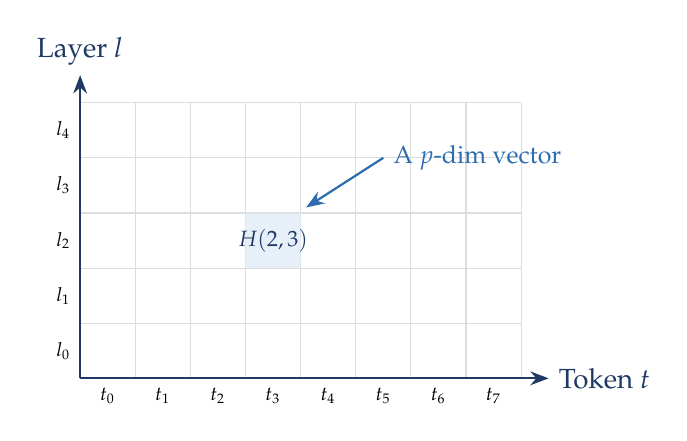
\begin{tikzpicture}[scale=0.7]
  % Grid
  \draw[step=1, MGray, thin] (0,0) grid (8,5);
  % Axes
  \draw[-{Stealth}, thick, Navy] (0,0) -- (8.5,0) node[right] {Token $t$};
  \draw[-{Stealth}, thick, Navy] (0,0) -- (0,5.5) node[above] {Layer $l$};
  % Labels
  \foreach \x in {0,...,7} \node[below, font=\scriptsize] at (\x+0.5, 0) {$t_{\x}$};
  \foreach \y in {0,...,4} \node[left, font=\scriptsize] at (0, \y+0.5) {$l_{\y}$};
  % A highlighted cell
  \fill[LBlue, opacity=0.7] (3,2) rectangle (4,3);
  \node[font=\footnotesize, Navy] at (3.5, 2.5) {$H(2,3)$};
  % Arrow pointing to it
  \draw[-{Stealth}, thick, Blue] (5.5, 4) -- (4.1, 3.1)
    node[pos=0, right, font=\small, Blue] {A $p$-dim vector};
\end{tikzpicture}
\end{center}

We call this the \textbf{layer--time grid}. ``Layer'' is the vertical axis
(depth in the network). ``Time'' is the horizontal axis (position in the
sequence). Every cell holds a $p$-dimensional vector.

\begin{keyidea}
The hidden states of a transformer form a \textbf{field} on a
two-dimensional grid. The geometry of this field---how vectors change across
layers and across tokens---reveals the model's internal computation.
\end{keyidea}

\section{The four big ideas}

This book develops four main ideas, each building on the last:

\begin{enumerate}
\item \textbf{Standardise the vectors} (Chapter~\ref{chap:whitening}).
  Raw hidden states have correlated, differently-scaled dimensions.
  We fix this with PCA-based whitening, like standardising variables
  before running a regression.

\item \textbf{Measure how vectors change} (Chapters~\ref{chap:kernels}--\ref{chap:curvature}).
  We decompose the layer-to-layer transformation into a rotation
  (direction change) and a stretch (magnitude change), then measure
  curvature---how much the grid's geometry twists.

\item \textbf{Run controlled experiments} (Chapter~\ref{chap:experiments}).
  We use factorial experimental design (DOE) to test which input
  properties actually affect the geometry: task type? reasoning
  difficulty? prompt length?

\item \textbf{Connect geometry to reasoning} (Chapter~\ref{chap:reasoning}).
  We add a new observable---\emph{dependency}---that measures how much
  each layer's hidden state matters for the model's final output.
  This lets us define reasoning, memory, and control in geometric terms.
\end{enumerate}

\begin{center}
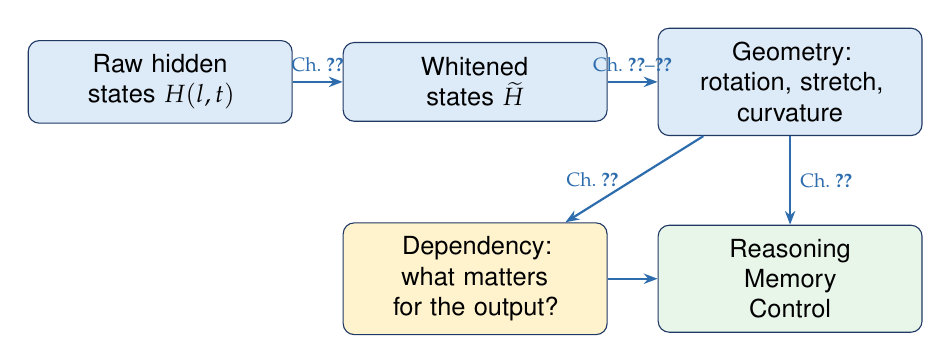
\begin{tikzpicture}[
  box/.style={draw=Navy, fill=LBlue, rounded corners=4pt,
              minimum height=1cm, text width=3cm, align=center,
              font=\small\sffamily, inner sep=5pt},
  arr/.style={-{Stealth[length=5pt]}, thick, Blue},
]
\node[box] (a) at (0,0) {Raw hidden\\states $H(l,t)$};
\node[box] (b) at (4,0) {Whitened\\states $\widetilde{H}$};
\node[box] (c) at (8,0) {Geometry:\\rotation, stretch,\\curvature};
\node[box, fill=LAmber] (d) at (4,-2.5) {Dependency:\\what matters\\for the output?};
\node[box, fill=LGreen] (e) at (8,-2.5) {Reasoning\\Memory\\Control};
\draw[arr] (a) -- (b) node[midway, above, font=\scriptsize] {Ch.~\ref{chap:whitening}};
\draw[arr] (b) -- (c) node[midway, above, font=\scriptsize] {Ch.~\ref{chap:kernels}--\ref{chap:curvature}};
\draw[arr] (c) -- (e) node[midway, right, font=\scriptsize] {Ch.~\ref{chap:reasoning}};
\draw[arr] (c) -- (d) node[midway, left, font=\scriptsize, xshift=-2pt] {Ch.~\ref{chap:reasoning}};
\draw[arr] (d) -- (e);
\end{tikzpicture}
\end{center}

\section{What you will be able to do}

By the end of this book, you will be able to:

\begin{itemize}[nosep]
\item Extract and whitened hidden states from any Hugging Face transformer.
\item Compute the polar decomposition of layer transitions and interpret
  what rotation and stretching mean.
\item Measure curvature and identify where in the network non-trivial
  computation happens.
\item Design and analyse factorial experiments on geometric quantities.
\item Compute dependency profiles that show which layers matter most
  for the model's output.
\item Diagnose specific failure modes (hallucination, instruction-ignoring,
  reasoning errors) using geometric signatures.
\end{itemize}

\section{Hands-on: your first analysis in 60 seconds}

\begin{lstlisting}[caption={Complete first analysis using the ltg library}]
import ltg

# Step 1: Load the model (takes ~30 seconds, only do this once)
model = ltg.load_model("Qwen/Qwen2.5-7B")

# Step 2: Analyse a prompt (takes ~10 seconds)
result = ltg.analyse("What is the square root of 144?", model=model)

# Step 3: See the summary
result.summary()
# Output:
#   Tokens: 9  |  Layers: 28  |  Whitened dim: 256
#   Mean curvature: 0.0847
#   Peak layer: 26 (of 27)
#   Final-3-layer share: 42.3%
#   ...

# Step 4: Generate all plots
result.plot_all(prefix="ch1_first")
# Creates: ch1_first_curvature.png, ch1_first_kernel.png,
#          ch1_first_polar.png, ch1_first_dependency.png
\end{lstlisting}

\begin{tryit}
Run the code above. Then try two more prompts:
\begin{itemize}[nosep]
\item A factual question: \texttt{"Who wrote Romeo and Juliet?"}
\item A reasoning problem: \texttt{"If all cats are animals and Whiskers is a cat, what is Whiskers?"}
\end{itemize}
Compare the three summaries. Which has the highest curvature? Which has the
lowest dependency entropy? Do the differences surprise you?
\end{tryit}


% ══════════════════════════════════════════════════════════════════════════════
\chapter{Standardising the Internal Representation}
\label{chap:whitening}
% ══════════════════════════════════════════════════════════════════════════════

\notebook{ch2\_whitening.ipynb}

\begin{whycare}
If you compare hidden states at different layers without standardising them
first, you are comparing apples and oranges. Whitening is to hidden-state
analysis what z-scoring is to statistical analysis: it removes scale
differences and correlations so that the geometry you measure is real, not an
artefact of the coordinate system.
\end{whycare}

\section{The problem with raw hidden states}

A transformer's hidden state vector has $p$ dimensions (typically 2048--8192).
These dimensions are \emph{not} independent:
\begin{itemize}[nosep]
\item Some dimensions carry much more variance than others.
\item Many dimensions are correlated.
\item The scale changes from layer to layer.
\end{itemize}

If you directly compute distances between hidden states at different layers,
the distance is dominated by whichever dimensions happen to have the largest
variance---not necessarily the most informative ones.

\begin{analogy}
Imagine measuring the similarity between cities using two features: population
(in millions) and average temperature (in degrees). Population ranges from
0.01 to 30; temperature ranges from $-20$ to $45$. Without standardisation,
Euclidean distance is almost entirely determined by population, and temperature
barely matters. The same problem occurs in hidden states, but with thousands
of dimensions.
\end{analogy}

\section{The solution: PCA-based whitening}

The fix is a standard statistical tool: \textbf{whitening via PCA}.

\textbf{Step 1: Centre.} Subtract the mean hidden state $\bar{H}$ computed
across all layers and tokens for a given input.

\textbf{Step 2: Compute the covariance.} The $p \times p$ covariance matrix
$\Sigma$ captures how dimensions co-vary.

\textbf{Step 3: PCA projection.} Take the top $k$ eigenvectors
$V_k = [v_1, \ldots, v_k]$ of $\Sigma$, with eigenvalues
$\lambda_1 \geq \cdots \geq \lambda_k > 0$.

\textbf{Step 4: Whiten.} Define the whitening matrix
$W = V_k \,\text{diag}(\lambda_1^{-1/2}, \ldots, \lambda_k^{-1/2})$
and compute:
\[
  \widetilde{H}(l,t) = \bigl(H(l,t) - \bar{H}\bigr) \, W
  \quad \in \mathbb{R}^k
\]

The result: $\widetilde{H}$ has uncorrelated dimensions with unit variance.
We use $k = 256$ throughout---this retains the meaningful variation while
making computation tractable.

\begin{keyidea}
After whitening, Euclidean distance in the $k$-dimensional space equals
Mahalanobis distance in the original $p$-dimensional space. This means the
geometry we measure respects the model's internal metric, not an arbitrary
coordinate choice.
\end{keyidea}

\section{Why this matters: metric consistency}

The core theoretical result (proven formally in the research monograph) is:

\begin{tcolorbox}[base, colback=LGreen, colframe=DGreen]
\textbf{Metric Consistency Theorem (informal).}
After whitening, the covariance of the hidden states is the identity matrix.
All subsequent geometric operations---decompositions, distances,
curvatures---are invariant to the original coordinate system of the model.
\end{tcolorbox}

In plain language: whitening lets us compare geometry \emph{across layers,
across prompts, and across models} in a principled way. Without it, we would
be measuring artefacts.

\section{Python implementation}

\begin{lstlisting}[caption={Whitening hidden states from a Hugging Face model}]
import torch
from transformers import AutoModelForCausalLM, AutoTokenizer

def extract_and_whiten(model, tokenizer, text, k=256):
    """Extract whitened hidden states from a transformer."""
    inputs = tokenizer(text, return_tensors="pt").to(model.device)

    with torch.no_grad():
        out = model(**inputs, output_hidden_states=True)

    # Stack all layers: shape (L+1, T, p)
    H = torch.stack(out.hidden_states)     # includes layer 0
    H = H[1:]                               # skip embedding layer
    L, T, p = H.shape

    # Step 1: Centre
    H_flat = H.reshape(-1, p)               # (L*T, p)
    H_mean = H_flat.mean(dim=0)
    H_centred = H_flat - H_mean

    # Step 2-3: PCA via SVD
    U, S, Vt = torch.linalg.svd(H_centred, full_matrices=False)
    V_k = Vt[:k].T                          # (p, k)
    eigenvalues = (S[:k] ** 2) / (L * T - 1)

    # Step 4: Whiten
    W = V_k * (1.0 / eigenvalues.sqrt())    # (p, k)
    H_whitened = H_centred @ W              # (L*T, k)
    H_whitened = H_whitened.reshape(L, T, k)

    return H_whitened  # shape: (L, T, k)
\end{lstlisting}

\section{Using the ltg library}

The \texttt{ltg.analyse()} function performs whitening automatically. But you
can inspect the whitened states directly:

\begin{lstlisting}[caption={Inspecting whitened hidden states with ltg}]
import ltg
import numpy as np

model = ltg.load_model("Qwen/Qwen2.5-7B")
result = ltg.analyse("The capital of France is", model=model)

# Access the whitened hidden states
H_w = result.H_whitened  # shape: (L, T, k)
print(f"Shape: {H_w.shape}")
# e.g., Shape: (28, 7, 256)

# Verify whitening: covariance should be close to identity
H_flat = H_w.reshape(-1, H_w.shape[2])  # (L*T, k)
cov = np.cov(H_flat.T)                   # (k, k)

# Check: diagonal should be ~1, off-diagonal should be ~0
print(f"Mean diagonal:     {np.diag(cov).mean():.4f}")   # ~1.0
print(f"Mean off-diagonal: {np.abs(cov - np.diag(np.diag(cov))).mean():.6f}")  # ~0.0
print(f"Max off-diagonal:  {np.abs(cov - np.diag(np.diag(cov))).max():.4f}")
\end{lstlisting}

\begin{tryit}
\textbf{Exercise 2.1:} Run the code above and verify the covariance is
approximately $I_k$.

\textbf{Exercise 2.2 (Whitening dimension):} Try $k = 32, 64, 128, 256$.
For each, compute the curvature profile and check whether the shape changes.
At what $k$ does the profile stabilise?
\begin{lstlisting}
# Hint: use the core library directly for custom k
import layer_time_geometry as core

for k in [32, 64, 128, 256]:
    H_raw = core.extract_hidden_states(model.hf_model, model.tokenizer,
                                        "The capital of France is", "cuda")
    H_np = H_raw[1:].cpu().numpy()
    metric = core.estimate_metric(H_np, n_components=k)
    H_w = core.whiten(H_np, metric)
    Omega = core.curvature(H_w)
    print(f"k={k:3d}: mean_curv={Omega.mean():.4f}, "
          f"peak_layer={Omega.mean(axis=1).argmax()}")
\end{lstlisting}
\end{tryit}

\section{What we skip on first reading}

The research monograph proves several additional properties: that whitening
is the unique linear transformation achieving metric consistency, that the
effective rank of the covariance determines the intrinsic dimensionality,
and that the choice of $k$ is stable for $k \geq 128$.

\begin{pitfall}
\textbf{Do not skip layer 0.} Layer~0 is the raw token embedding before any
transformer processing. Including it in the whitening distorts the geometry
because it has a fundamentally different distribution. Always start from
layer~1. The \texttt{ltg} library handles this automatically.
\end{pitfall}


% ══════════════════════════════════════════════════════════════════════════════
\chapter{Measuring Similarity: Kernels on the Grid}
\label{chap:kernels}
% ══════════════════════════════════════════════════════════════════════════════

\notebook{ch3\_kernels.ipynb}

\begin{whycare}
Kernels answer the most basic question about the hidden-state grid: which
layers are similar to each other? Which token positions are similar? The
answers reveal the model's computational phases---setup, processing,
and decision-making.
\end{whycare}

\section{What is a kernel?}

A kernel is just a similarity function. Given two objects $a$ and $b$, a
kernel $K(a, b)$ returns a number indicating how similar they are. You already
know several kernels:

\begin{itemize}[nosep]
\item \textbf{Dot product}: $K(a, b) = a^\top b$ --- the simplest kernel.
\item \textbf{Cosine similarity}: $K(a, b) = \frac{a^\top b}{\|a\|\|b\|}$
  --- normalised dot product.
\item \textbf{RBF kernel}: $K(a, b) = \exp(-\|a - b\|^2 / 2\sigma^2)$
  --- similarity decays with distance.
\end{itemize}

We define two kernels on the layer--time grid.

\section{The layer kernel: which layers are similar?}

For each layer $l$, collect all $T$ whitened token vectors into a matrix
$\widetilde{H}^{(l)} \in \mathbb{R}^{T \times k}$. The \textbf{layer kernel}
measures how similar two layers are:
\[
  K_{\text{layer}}(l, l') = \frac{1}{T}
  \operatorname{tr}\!\left(
    \widetilde{H}^{(l)\top} \widetilde{H}^{(l')}
  \right)
\]
This is just the average dot product between corresponding token vectors at
two layers.

\begin{analogy}
Think of each layer as a photograph of the assembly line taken from above.
The layer kernel measures how much two photographs look alike. Early layers
look similar to each other (setup phase), late layers look similar to each
other (decision phase), and there is often a visible transition in the
middle (processing phase).
\end{analogy}

\section{The temporal kernel: which tokens are similar?}

Similarly, for each token $t$, collect its representation across all layers:
$\widetilde{H}_t \in \mathbb{R}^{L \times k}$. The \textbf{temporal kernel}
measures:
\[
  K_{\text{time}}(t, t') = \frac{1}{L}
  \operatorname{tr}\!\left(
    \widetilde{H}_t^\top \widetilde{H}_{t'}
  \right)
\]

\section{What the kernels reveal: three computational phases}

\begin{finding}
When we compute the layer kernel for typical prompts across multiple models
(Qwen2.5-7B, DeepSeek-R1-7B, Qwen2.5-32B), we consistently find
\textbf{three phases}:

\begin{enumerate}[nosep]
\item \textbf{Early layers} ($l \lesssim L/4$): High mutual similarity.
  The model is building up basic representations.
\item \textbf{Middle layers} ($L/4 \lesssim l \lesssim 3L/4$): Rapid change.
  This is where the ``work'' happens---attention heads route
  information, representations diverge.
\item \textbf{Late layers} ($l \gtrsim 3L/4$): Convergence toward a
  prediction-ready state. Curvature peaks here.
\end{enumerate}
\end{finding}

\begin{lstlisting}[caption={Computing the layer kernel matrix}]
def layer_kernel(H_whitened):
    """Compute the L x L layer kernel matrix.

    Args:
        H_whitened: tensor of shape (L, T, k)
    Returns:
        K: tensor of shape (L, L)
    """
    L, T, k = H_whitened.shape
    # Reshape to (L, T*k) and compute normalised Gram matrix
    H_flat = H_whitened.reshape(L, T * k)
    K = H_flat @ H_flat.T / T
    return K
\end{lstlisting}

\section{Hands-on: visualising the three phases}

\begin{lstlisting}[caption={Visualising the layer kernel to see computational phases}]
import ltg

model = ltg.load_model("Qwen/Qwen2.5-7B")
result = ltg.analyse("Explain why the sky is blue", model=model)

# The layer kernel is already computed
result.plot_layer_kernel(save_path="ch3_kernel.png")

# You will see a block-diagonal structure:
#   - Top-left block (early layers): high similarity
#   - Middle: transition zone
#   - Bottom-right block (late layers): high similarity
# The transition boundary marks where the model shifts
# from "understanding" to "deciding".
\end{lstlisting}

\begin{tryit}
\textbf{Exercise 3.1:} Compare layer kernels for a short prompt (5 tokens)
and a long prompt (50+ tokens). Does the three-phase structure hold for both?

\textbf{Exercise 3.2 (Phase boundary detection):} The phase boundary is
where consecutive layer similarity drops. Write code to find it:
\begin{lstlisting}
K = result.layer_kernel_matrix
# Consecutive similarity: K[l, l+1] for each l
consec = [K[l, l+1] for l in range(K.shape[0] - 1)]
import numpy as np
transition = np.argmin(consec)
print(f"Phase transition at layer {transition}")
\end{lstlisting}
Where does the transition occur relative to the total depth?
\end{tryit}


% ══════════════════════════════════════════════════════════════════════════════
\chapter{How Information Flows: Operators and Polar Decomposition}
\label{chap:operators}
% ══════════════════════════════════════════════════════════════════════════════

\notebook{ch4\_polar\_decomposition.ipynb}

\begin{whycare}
This is the chapter where the framework becomes powerful. We decompose
\emph{how} hidden states change from one layer to the next into two
fundamental operations: rotation and stretching. This decomposition is
the key to understanding what each layer actually does.
\end{whycare}

\section{The layer transition operator}

Between layer $l$ and layer $l+1$, the hidden states change. We can
approximate this change with a linear operator $T^{(l)}$ that best maps
$\widetilde{H}^{(l)}$ to $\widetilde{H}^{(l+1)}$:
\[
  \widetilde{H}^{(l+1)} \approx \widetilde{H}^{(l)} \, T^{(l)}
\]

We find $T^{(l)}$ by ordinary least squares---the same linear regression
you learned in your first statistics course, just applied to matrices:
\[
  T^{(l)} = \left(\widetilde{H}^{(l)\top}\widetilde{H}^{(l)}\right)^{-1}
  \widetilde{H}^{(l)\top}\widetilde{H}^{(l+1)}
\]

\begin{analogy}
If the hidden states at layer $l$ are the ``input data'' and the hidden
states at layer $l+1$ are the ``output data'', then $T^{(l)}$ is the
best linear predictor. It tells us: what linear transformation best
explains how the representation changed?
\end{analogy}

\section{Polar decomposition: rotation + stretch}

Every square matrix can be decomposed as:
\[
  T^{(l)} = U^{(l)} \, P^{(l)}
\]
where:
\begin{itemize}[nosep]
\item $U^{(l)}$ is an \textbf{orthogonal matrix} (rotation/reflection):
  it changes directions without changing magnitudes.
\item $P^{(l)}$ is a \textbf{symmetric positive-definite matrix}
  (stretching): it scales different directions by different amounts.
\end{itemize}

This is called the \textbf{polar decomposition}, and it is analogous to
writing a complex number as $z = e^{i\theta} \cdot r$ (angle + magnitude).

\begin{keyidea}
Every layer transition in a transformer does two things:
\begin{enumerate}[nosep]
\item \textbf{Rotate} the representation (change which directions are
  active), captured by $U^{(l)}$.
\item \textbf{Stretch} the representation (amplify some directions,
  compress others), captured by $P^{(l)}$.
\end{enumerate}
These are the two fundamental primitives of transformer computation.
\end{keyidea}

\section{What rotation and stretching mean}

\begin{center}
\renewcommand{\arraystretch}{1.5}
\begin{tabular}{@{}L{2cm} L{4cm} L{4.5cm}@{}}
\toprule
\textbf{Component} & \textbf{What it does} & \textbf{Computational meaning} \\
\midrule
$U^{(l)}$ (rotation) &
  Rotates the coordinate axes; preserves all distances &
  Attention mixing: redistributes information across directions without
  losing or amplifying anything \\
$P^{(l)}$ (stretch) &
  Stretches some directions, compresses others &
  Feature selection: amplifies important directions, suppresses
  irrelevant ones \\
\bottomrule
\end{tabular}
\end{center}

\section{Measuring the stretch: eigenvalues of P}

The eigenvalues $\sigma_1 \geq \sigma_2 \geq \cdots \geq \sigma_k$ of
$P^{(l)}$ tell us how much each principal direction is stretched:

\begin{itemize}[nosep]
\item $\sigma_i > 1$: direction $i$ is amplified (the model is paying
  more attention to this direction).
\item $\sigma_i < 1$: direction $i$ is compressed (the model is
  discarding information along this direction).
\item $\sigma_i = 1$: direction $i$ is unchanged.
\end{itemize}

The \textbf{condition number} $\kappa = \sigma_1 / \sigma_k$ measures how
selective the layer is. A high condition number means the layer strongly
amplifies some directions while crushing others---it is making a sharp
``decision''.

The \textbf{effective rank} $\text{erank} = \exp(H(\hat\sigma))$, where
$H$ is the entropy of the normalised eigenvalue distribution, measures how
many directions are actively used. Low effective rank means the layer
concentrates its computation in a few directions.

\begin{lstlisting}[caption={Polar decomposition of layer transitions}]
def polar_decompose_layers(H_whitened):
    """Compute polar decomposition T = U @ P for each layer.

    Args:
        H_whitened: (L, T, k) whitened hidden states
    Returns:
        Us: list of L-1 orthogonal matrices (k, k)
        Ps: list of L-1 symmetric positive-definite matrices (k, k)
    """
    L, T, k = H_whitened.shape
    Us, Ps = [], []

    for l in range(L - 1):
        H_l = H_whitened[l]       # (T, k)
        H_next = H_whitened[l+1]  # (T, k)

        # Least-squares transition operator
        T_l = torch.linalg.lstsq(H_l, H_next).solution  # (k, k)

        # Polar decomposition
        U, S, Vt = torch.linalg.svd(T_l)
        P = Vt.T @ torch.diag(S) @ Vt   # symmetric positive-definite
        U_orth = U @ Vt                   # orthogonal
        Us.append(U_orth)
        Ps.append(P)

    return Us, Ps
\end{lstlisting}

\section{Hands-on: exploring the polar decomposition with ltg}

The \texttt{ltg} library computes the polar decomposition automatically. You
can visualise it and inspect individual layers:

\begin{lstlisting}[caption={Polar decomposition analysis with ltg}]
import ltg
import numpy as np

model = ltg.load_model("Qwen/Qwen2.5-7B")
result = ltg.analyse("If x = 3 and y = 2*x + 1, what is y?", model=model)

# Plot condition number and effective rank across layers
result.plot_polar(save_path="ch4_polar.png")

# Inspect a specific layer's stretch
layer = 25  # a late layer
P = result.polar_P[layer]             # (k, k) symmetric matrix
sigmas = np.linalg.svd(P, compute_uv=False)  # eigenvalues

print(f"Layer {layer} stretch spectrum:")
print(f"  Top 5 eigenvalues:    {sigmas[:5]}")
print(f"  Bottom 5 eigenvalues: {sigmas[-5:]}")
print(f"  Condition number:     {sigmas[0]/sigmas[-1]:.1f}")
print(f"  Effective rank:       {result.effective_ranks[layer]:.1f}")
# High condition number = the layer is being very selective
# Low effective rank = computation concentrates in few directions
\end{lstlisting}

\begin{tryit}
\textbf{Exercise 4.1 (Rotation vs.\ stretch magnitude):} For each layer, compute:
\begin{itemize}[nosep]
\item $\|U^{(l)} - I\|_F$ (how much rotation deviates from identity)
\item $\|P^{(l)} - I\|_F$ (how much stretching deviates from identity)
\end{itemize}
\begin{lstlisting}
for l in range(result.n_layers - 1):
    U_dev = np.linalg.norm(result.polar_U[l] - np.eye(result.k), 'fro')
    P_dev = np.linalg.norm(result.polar_P[l] - np.eye(result.k), 'fro')
    print(f"Layer {l:2d}: rotation={U_dev:.3f}, stretch={P_dev:.3f}")
\end{lstlisting}
Which layers have more rotation? Which have more stretching? Is there a pattern?

\textbf{Exercise 4.2 (Compare tasks):} Analyse an arithmetic prompt and a
factual retrieval prompt. Compare their condition number profiles. Does the
model make sharper ``decisions'' for one task type?
\end{tryit}


% ══════════════════════════════════════════════════════════════════════════════
\chapter{Where the Action Is: Curvature}
\label{chap:curvature}
% ══════════════════════════════════════════════════════════════════════════════

\notebook{ch5\_curvature.ipynb}

\begin{whycare}
Curvature tells you \emph{where} in the layer--time grid the interesting
computation happens. Zero curvature means the model could be replaced by
a simple linear transformation at that point. High curvature means something
genuinely non-trivial is occurring. This is the single most useful
diagnostic in the framework.
\end{whycare}

\section{The idea of curvature on a grid}

In everyday life, curvature measures how much a surface bends. A flat table
has zero curvature. A basketball has constant positive curvature. A saddle
has negative curvature.

On the layer--time grid, curvature measures something analogous: how much
the geometry ``twists'' when you go around a small loop.

\begin{analogy}
Imagine walking around a square block in a city. You make four right turns
and end up facing the same direction---zero curvature. Now imagine walking
the same square on the surface of a sphere (like walking a small square near
the North Pole). After four right turns, you \emph{do not} face the same
direction---the surface's curvature rotated you. The same idea applies to
hidden states: go right one token, go up one layer, go left one token,
go down one layer. If you end up with a different transformation than the
identity, there is curvature.
\end{analogy}

\section{Computing curvature on the layer--time grid}

Consider a small square (``plaquette'') at position $(l, t)$ on the grid:

\begin{center}
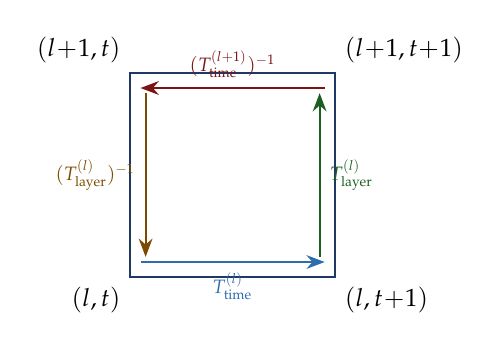
\begin{tikzpicture}[scale=1.3]
  \draw[thick, Navy] (0,0) rectangle (2,2);
  \node[below left, font=\small] at (0,0) {$(l,t)$};
  \node[below right, font=\small] at (2,0) {$(l,t\!+\!1)$};
  \node[above right, font=\small] at (2,2) {$(l\!+\!1,t\!+\!1)$};
  \node[above left, font=\small] at (0,2) {$(l\!+\!1,t)$};
  \draw[-{Stealth}, thick, Blue] (0.1, 0.15) -- (1.9, 0.15)
    node[midway, below, font=\scriptsize] {$T^{(l)}_{\text{time}}$};
  \draw[-{Stealth}, thick, DGreen] (1.85, 0.2) -- (1.85, 1.8)
    node[midway, right, font=\scriptsize] {$T^{(l)}_{\text{layer}}$};
  \draw[-{Stealth}, thick, DRed] (1.9, 1.85) -- (0.1, 1.85)
    node[midway, above, font=\scriptsize] {$(T^{(l+1)}_{\text{time}})^{-1}$};
  \draw[-{Stealth}, thick, Amber] (0.15, 1.8) -- (0.15, 0.2)
    node[midway, left, font=\scriptsize] {$(T^{(l)}_{\text{layer}})^{-1}$};
\end{tikzpicture}
\end{center}

Going around this loop gives a combined transformation:
\[
  \Omega(l, t) = T^{(l)}_{\text{time}} \cdot T^{(l)}_{\text{layer}}
  \cdot \left(T^{(l+1)}_{\text{time}}\right)^{-1}
  \cdot \left(T^{(l)}_{\text{layer}}\right)^{-1}
\]

If the grid were ``flat'' (i.e., moving right then up gives the same result
as moving up then right), then $\Omega(l,t) = I$. The deviation from
identity \emph{is} the curvature:
\[
  \text{curvature at } (l,t) = \|\Omega(l,t) - I\|_F
\]
where $\|\cdot\|_F$ is the Frobenius norm (think: sum of squared entries,
then square root).

\begin{keyidea}
Curvature measures \textbf{non-commutativity}: does it matter whether you
go ``right then up'' or ``up then right'' on the grid? If yes, the
computation at that point is genuinely nonlinear and non-trivial.
\end{keyidea}

\section{What curvature tells us}

\begin{finding}
Across all models tested (three architectures, two scales), curvature
consistently shows the same pattern:

\begin{itemize}[nosep]
\item \textbf{Early layers}: Low curvature. The model is doing simple,
  nearly-linear processing.
\item \textbf{Middle layers}: Moderate curvature. Information routing
  and mixing.
\item \textbf{Final 3--5 layers}: Curvature spikes sharply. This is
  where the model commits to its prediction.
\end{itemize}

This is the most robust finding in the entire framework---it replicates
across models, prompts, and tasks.
\end{finding}

\begin{pitfall}
\textbf{Curvature does not equal reasoning complexity.} Early in this
research, we conjectured that higher curvature meant harder reasoning.
Controlled experiments across three models showed this is \textbf{false}:
reasoning depth (number of logical steps) has no significant effect on
curvature. Curvature measures \emph{non-separable interaction} between
layers and tokens---not how ``hard'' the model is thinking.
\end{pitfall}

\section{Hands-on: curvature maps with ltg}

\begin{lstlisting}[caption={Curvature analysis with ltg}]
import ltg

model = ltg.load_model("Qwen/Qwen2.5-7B")

# Analyse two prompts of different "difficulty"
r_easy = ltg.analyse("What is 2 + 2?", model=model)
r_hard = ltg.analyse(
    "If f(x) = 3x^2 - 2x + 1, what is f'(x) evaluated at x = 4?",
    model=model
)

# Plot curvature maps for both
r_easy.plot_curvature(save_path="ch5_curv_easy.png")
r_hard.plot_curvature(save_path="ch5_curv_hard.png")

# Compare them side by side
ltg.compare([r_easy, r_hard], save_path="ch5_compare.png")

# Print summaries
print("Easy prompt:")
print(f"  Peak curvature layer: {r_easy.curvature_by_layer.argmax()}")
print(f"  Final-3-layer share:  "
      f"{r_easy.curvature_by_layer[-3:].sum()/r_easy.curvature_by_layer.sum():.1%}")
print("Hard prompt:")
print(f"  Peak curvature layer: {r_hard.curvature_by_layer.argmax()}")
print(f"  Final-3-layer share:  "
      f"{r_hard.curvature_by_layer[-3:].sum()/r_hard.curvature_by_layer.sum():.1%}")
# Key finding: the peak location is similar! Curvature does NOT
# increase with problem difficulty.
\end{lstlisting}

\begin{tryit}
\textbf{Exercise 5.1 (Testing the negative result):} Analyse five prompts
with increasing reasoning depth (1-step, 2-step, \ldots, 5-step). Plot
their mean curvature. Does it increase? (Spoiler: it should not.)

\textbf{Exercise 5.2 (Curvature across models):} If you have access to
a second model (e.g., \texttt{Qwen/Qwen2.5-1.5B}), compare curvature
profiles on the same prompt. Does the three-phase structure persist at
smaller scale?
\end{tryit}


% ╔════════════════════════════════════════════════════════════════════════════╗
\part{What Do the Experiments Say?}
% ╚════════════════════════════════════════════════════════════════════════════╝


% ══════════════════════════════════════════════════════════════════════════════
\chapter{Testing What Matters: Experimental Design}
\label{chap:experiments}
% ══════════════════════════════════════════════════════════════════════════════

\notebook{ch6\_experiments.ipynb}

\begin{whycare}
Anyone can compute a metric. The hard part is knowing whether the metric
actually tells you something about the input. Experimental design (DOE) is
the tool that separates real signal from noise. This chapter uses the same
factorial designs you learn in statistics courses---applied to transformer
geometry.
\end{whycare}

\section{The experimental setup}

We designed 320 prompts varying five factors:

\begin{center}
\renewcommand{\arraystretch}{1.4}\small
\begin{tabular}{@{}L{3cm} L{6cm}@{}}
\toprule
\textbf{Factor} & \textbf{Levels} \\
\midrule
Cognitive task & Arithmetic, Deductive Reasoning, Causal Reasoning,
  Linguistic Analysis, Factual Retrieval, Definition \\
Reasoning depth & Low (1-step), Medium (2-3 steps), High (4+ steps) \\
Prompt length & Short ($<$50 tokens), Medium, Long ($>$150 tokens) \\
Knowledge domain & Science, History, Everyday, Abstract \\
Robustness & Original, Paraphrased \\
\bottomrule
\end{tabular}
\end{center}

For each prompt, we extracted whitened hidden states and computed $\sim$20
geometric metrics (curvature, condition number, effective rank, dependency
measures, etc.). Then we ran ANOVA: which factors significantly affect which
metrics?

\section{Three models}

We ran the experiment on three models to check replicability:

\begin{center}
\renewcommand{\arraystretch}{1.3}
\begin{tabular}{@{}lll@{}}
\toprule
\textbf{Model} & \textbf{Parameters} & \textbf{Layers} \\
\midrule
Qwen2.5-7B & 7 billion & 28 \\
DeepSeek-R1-Distill-Qwen-7B & 7 billion & 28 \\
Qwen2.5-32B & 32 billion & 64 \\
\bottomrule
\end{tabular}
\end{center}

\section{The results: five key findings}

\begin{finding}
\textbf{R1: Task type matters, but modestly.}

Cognitive task type (arithmetic vs.\ reasoning vs.\ retrieval, etc.) is
\emph{detectable} in the geometry---certain dependency metrics differ
significantly across task types. But the effect sizes are small
($\eta^2 \approx 0.02$--$0.05$). Task type is a real signal, not the
dominant driver.
\end{finding}

\begin{finding}
\textbf{R2: Surface features are not negligible.}

We expected that ``shallow'' features like prompt length and formatting would
have no effect on geometry. \textbf{Wrong.} Prompt length affects dependency
horizons significantly, especially in DeepSeek-R1. Robustness condition
drives the largest single effect in Qwen-7B ($\eta^2 = 0.098$ for the
global curvature ratio). The geometry responds to both computational content
\emph{and} input form.
\end{finding}

\begin{finding}
\textbf{R3: Reasoning depth has no effect on geometry.}

This is the cleanest and most important negative result. Across all three
models, the factor ``reasoning depth'' (1-step vs.\ multi-step problems)
\emph{fails to reach significance} on any geometric metric. The one minor
exception: condition number in Qwen-7B ($\eta^2 = 0.032$, $p = 0.010$).

\textbf{What this means:} you cannot tell how many reasoning steps a problem
requires by looking at the geometry of the hidden states. The number of
logical steps does not map to any measurable internal geometric quantity.
\end{finding}

\begin{finding}
\textbf{R4: Curvature concentrates in the final layers.}

This finding replicates unanimously across all three models. In Qwen2.5-32B
(64 layers), peak curvature is entirely in the final 3 layers. This is the
most robust qualitative finding in the study.
\end{finding}

\begin{finding}
\textbf{R5: Dependency tracks task type more closely than curvature.}

Dependency-based metrics (how much each layer's state matters for the output)
are more sensitive to task type than curvature-based metrics. They are also
more stable under paraphrase.
\end{finding}

\begin{center}
\renewcommand{\arraystretch}{1.4}\small
\begin{tabular}{@{}L{4.5cm} C{1.5cm} C{1.5cm} C{1.5cm}@{}}
\toprule
\rowcolor{Navy}
\textcolor{white}{\textbf{Finding}} &
\textcolor{white}{\textbf{Qwen-7B}} &
\textcolor{white}{\textbf{DS-R1}} &
\textcolor{white}{\textbf{Qwen-32B}} \\
\midrule
Task type detectable    & yes & yes & yes \\
Surface features weak   & \textbf{no} & \textbf{no} & \textbf{no} \\
Curvature = reasoning depth & \textbf{no} & \textbf{no} & \textbf{no} \\
Curvature in final layers   & yes & yes & yes \\
Dependency stable           & yes & yes & yes \\
\bottomrule
\end{tabular}
\end{center}

\section{Hands-on: your own mini-DOE}

You can replicate a small version of our experiment with \texttt{ltg}:

\begin{lstlisting}[caption={Mini factorial experiment with ltg}]
import ltg
import numpy as np
from scipy import stats

model = ltg.load_model("Qwen/Qwen2.5-7B")

# Define prompts by task type
prompts = {
    "arithmetic": [
        "What is 17 * 23?",
        "Calculate 156 / 12",
        "What is 2^10?",
    ],
    "reasoning": [
        "If all dogs are pets and Rex is a dog, is Rex a pet?",
        "If it rains then the ground is wet. The ground is wet. Did it rain?",
        "Alice is taller than Bob. Bob is taller than Carol. Who is shortest?",
    ],
    "retrieval": [
        "What is the capital of Japan?",
        "Who painted the Mona Lisa?",
        "What year did World War II end?",
    ],
}

# Collect metrics by task type
results_by_task = {}
for task, texts in prompts.items():
    metrics = []
    for text in texts:
        r = ltg.analyse(text, model=model, compute_dependency=True)
        metrics.append({
            'mean_curv': r.curvature_by_layer.mean(),
            'peak_layer': r.curvature_by_layer.argmax(),
            'dep_entropy': r.dep_entropy,
            'dep_h90': r.dep_horizon_90,
        })
    results_by_task[task] = metrics

# Simple one-way ANOVA on dependency entropy
groups = [
    [m['dep_entropy'] for m in results_by_task[t] if m['dep_entropy']]
    for t in prompts.keys()
]
F, p = stats.f_oneway(*groups)
print(f"ANOVA on dep_entropy: F={F:.3f}, p={p:.3f}")
print("Task type significant?" , "Yes" if p < 0.05 else "No")
\end{lstlisting}

\begin{tryit}
\textbf{Exercise 6.1:} Expand the mini-DOE to 5 prompts per task type and
add a fourth task (e.g., ``definition''). Run the ANOVA. Which metric shows
the strongest task-type effect?

\textbf{Exercise 6.2 (Paraphrase stability):} Take one prompt and create
three paraphrases. Analyse all four versions. How similar are their curvature
profiles? Compute the pairwise correlation.
\end{tryit}


% ══════════════════════════════════════════════════════════════════════════════
\chapter{What Each Layer Contributes: Dependency}
\label{chap:dependency}
% ══════════════════════════════════════════════════════════════════════════════

\notebook{ch7\_dependency.ipynb}

\begin{whycare}
Geometry tells you \emph{what shape} the hidden states have. Dependency tells
you \emph{which parts matter}. A layer might have complex geometry but
contribute nothing to the final output. Dependency distinguishes
``busy work'' from ``real work.''
\end{whycare}

\section{The idea}

After a model processes a prompt, it produces a score (log-probability) for
the next token. Some layers contributed heavily to this score; others barely
mattered. \textbf{Dependency} measures this contribution using gradients.

\begin{analogy}
In a relay race, some runners gain time and others lose time. The final
clock time depends on all runners, but not equally. Dependency is like
looking at the split times to figure out who actually made the difference.
\end{analogy}

\section{Computing dependency}

The dependency of layer $l$ is:
\[
  D_l = \left\|\frac{\partial s}{\partial \widetilde{H}^{(l)}}\right\|_F
\]
where $s$ is the model's score for the next token. This is just the
gradient of the output with respect to the hidden state at layer~$l$.
Layers where the gradient is large ``mattered more'' for the output.

\begin{lstlisting}[caption={Computing dependency profiles}]
def dependency_profile(model, tokenizer, text, k=256):
    """Compute dependency D_l for each layer."""
    inputs = tokenizer(text, return_tensors="pt").to(model.device)

    # Forward pass with gradient tracking
    out = model(**inputs, output_hidden_states=True)
    hidden_states = out.hidden_states[1:]  # skip layer 0

    # Score: log-prob of the predicted next token
    logits = out.logits[0, -1, :]          # last position
    score = logits.max()                    # score of top token

    # Backward pass
    score.backward()

    # Collect gradient norms per layer
    D = []
    for hs in hidden_states:
        if hs.grad is not None:
            D.append(hs.grad.norm().item())
        else:
            D.append(0.0)

    return D  # list of length L
\end{lstlisting}

\textbf{Note}: the code above is simplified. In practice, you need to enable
gradient computation for intermediate hidden states, which requires hooks.
See the research monograph's implementation appendix for the full version.

\section{Dependency profiles}

The dependency profile $D_0, D_1, \ldots, D_{L-1}$ reveals which layers
drive the output.

Useful summary statistics:
\begin{itemize}[nosep]
\item $D_{\text{total}} = \sum_l D_l$ --- total sensitivity to all layers.
\item \textbf{Dependency horizon} $H_\alpha$ --- the layer at which
  $\alpha\%$ of the total dependency is reached. A low $H_{90}$ means
  the model makes up its mind early.
\item \textbf{Dependency entropy} $S = -\sum_l \hat{D}_l \log \hat{D}_l$
  (where $\hat{D}_l = D_l / D_{\text{total}}$) --- how spread out the
  dependency is. High entropy = many layers contribute; low entropy = a
  few layers dominate.
\end{itemize}

\begin{pitfall}
\textbf{Length confound.} Total dependency $D_{\text{total}}$ is strongly
correlated with sequence length ($r \approx 0.96$). Longer sequences have
more hidden states for the gradient to flow through, mechanically increasing
$D_{\text{total}}$. Always use \textbf{normalised} metrics (entropy,
horizons, concentration ratios) when comparing prompts of different lengths.
\end{pitfall}

\section{Hands-on: dependency profiles with ltg}

\begin{lstlisting}[caption={Computing and visualising dependency profiles}]
import ltg
import numpy as np

model = ltg.load_model("Qwen/Qwen2.5-7B")

# Analyse with dependency (default: compute_dependency=True)
result = ltg.analyse(
    "The Pythagorean theorem states that a^2 + b^2 = c^2",
    model=model
)

# Plot the dependency profile
result.plot_dependency(save_path="ch7_dependency.png")

# Access the raw profile
D = result.dependency_profile
D_norm = D / D.sum()  # normalise

print(f"Total dependency:          {result.dep_total:.4f}")
print(f"Dependency entropy:        {result.dep_entropy:.3f}")
print(f"Horizon-90 (layer):        {result.dep_horizon_90}")
print(f"Final-3-layer concentration: {result.dep_concentration_final3:.1%}")

# Find the top-3 most important layers
top3 = np.argsort(D_norm)[-3:][::-1]
for l in top3:
    print(f"  Layer {l}: {D_norm[l]:.1%} of total dependency")
\end{lstlisting}

\begin{tryit}
\textbf{Exercise 7.1 (Length confound):} Analyse prompts of lengths 10, 30,
and 100 tokens. Plot $D_{\text{total}}$ vs.\ token count. Verify the
correlation. Then plot dependency \emph{entropy} vs.\ token count---is the
confound still present?

\textbf{Exercise 7.2 (Comparing dependency and curvature):} For a single
prompt, overlay the normalised curvature profile and the normalised
dependency profile on the same plot:
\begin{lstlisting}
import matplotlib.pyplot as plt
curv_norm = result.curvature_by_layer / result.curvature_by_layer.sum()
dep_norm = result.dependency_profile / result.dependency_profile.sum()
# Curvature has L-1 entries, dependency has L entries
plt.plot(curv_norm, label='Curvature (normalised)')
plt.plot(dep_norm, label='Dependency (normalised)')
plt.xlabel('Layer'); plt.legend()
plt.savefig('ch7_curv_vs_dep.png')
\end{lstlisting}
Do they peak at the same layers? What does it mean when curvature is high
but dependency is low?
\end{tryit}


% ╔════════════════════════════════════════════════════════════════════════════╗
\part{The Big Picture}
% ╚════════════════════════════════════════════════════════════════════════════╝


% ══════════════════════════════════════════════════════════════════════════════
\chapter{Reasoning, Memory, and Control}
\label{chap:reasoning}
% ══════════════════════════════════════════════════════════════════════════════

\notebook{ch8\_reasoning\_memory\_control.ipynb}

\begin{whycare}
This chapter connects everything. The geometry and dependency tools from
earlier chapters combine to give precise definitions of what it means for
a transformer to ``reason,'' ``remember,'' and be ``controlled.'' These are
not just philosophical labels---they have measurable signatures that you
can compute and test.
\end{whycare}

\section{Defining reasoning geometrically}

We all have intuitions about what ``reasoning'' means, but we need a
precise definition to measure it. Here is ours:

\begin{keyidea}
A transformer is \textbf{reasoning} at layer $l$ and token $t$ when three
conditions hold simultaneously:
\begin{enumerate}[nosep]
\item \textbf{Interaction}: The curvature $\|\Omega(l,t)\|$ is
  significantly above baseline---the model is doing non-trivial,
  nonlinear processing.
\item \textbf{Propagation}: The metric factor $P^{(l)}$ has high condition
  number---the model is selectively amplifying some directions.
\item \textbf{Dependency}: The dependency $D_{l,t}$ is high---the
  processing at this point actually matters for the output.
\end{enumerate}
All three must be present. Interaction without dependency is ``busy work.''
Dependency without interaction is just passing information through.
\end{keyidea}

\section{Defining memory}

The framework distinguishes two kinds of memory:

\textbf{Storage memory}: the model's weights encode facts
(``Paris is the capital of France''). This is a property of the parameters,
not the computation on a specific input.

\textbf{Functional memory}: information from early tokens persists and
influences the output at later layers. This \emph{is} a property of the
computation, and we measure it as \textbf{persistent dependency}:
\[
  \text{Pers}_\tau = \frac{D_\tau}{D_0}
\]
If a token from the beginning of the sequence ($\tau = 0$) still has high
dependency in the final layers, the model is ``remembering'' it functionally.

\section{Defining control}

Control means deliberately changing the model's computation by modifying
the geometry. The polar decomposition gives us two levers:

\begin{itemize}[nosep]
\item \textbf{Metric control}: clamping or modifying the eigenvalues
  of $P^{(l)}$ to change what the layer amplifies.
\item \textbf{Rotation control}: modifying $U^{(l)}$ to change the
  directions of information flow.
\end{itemize}

\subsection{The surprise: metric control dominates}

The research monograph originally predicted that combining rotation and
metric control (``dual control'') would work best, with rotation providing
the primary lever. The experiments showed the opposite:

\begin{finding}
\textbf{Metric control alone is sufficient.}

\begin{center}
\renewcommand{\arraystretch}{1.3}\small
\begin{tabular}{@{}lcc@{}}
\toprule
\textbf{Condition} & \textbf{Dep.\ total} & \textbf{Dep.\ entropy} \\
\midrule
Baseline & $\sim$1.00 & $\sim$2.45 \\
Rotation-only & $\sim$0.91 ($-$9\%) & $\sim$2.33 \\
Metric-only & $\sim$0.52 ($-$48\%) & $\sim$1.21 \\
Dual (both) & $\sim$0.52 ($-$48\%) & $\sim$1.21 \\
\bottomrule
\end{tabular}
\end{center}

Metric-only and dual control produce \emph{identical} results. Rotation
control adds nothing. The reason: the eigenvalue spectrum of $P^{(l)}$
directly controls how gradients flow, while rotation preserves norms and
therefore has little effect on gradient magnitudes.
\end{finding}

This is an important lesson: the theory predicted one thing, the data
showed another, and we updated the theory. Science works.

\section{Hands-on: running the control experiment yourself}

The \texttt{ltg} library provides a one-line control experiment:

\begin{lstlisting}[caption={Running the four-condition control study}]
import ltg

model = ltg.load_model("Qwen/Qwen2.5-7B")

# Run all four control conditions on a single prompt
results = ltg.control_experiment(
    "Explain why the sky appears blue during the day",
    model=model,
    metric_strength=0.5,    # how aggressively to clamp eigenvalues
    rotation_strength=0.3,  # how much to perturb rotation
)

# Print the results
print(f"{'Condition':15s} {'D_total':>8s} {'H_90':>5s} {'Entropy':>8s}")
print("-" * 40)
for name, r in results.items():
    print(f"{name:15s} {r.dep_total:8.3f} {r.dep_horizon_90:5d} "
          f"{r.dep_entropy:8.3f}")

# Visualise
ltg.plot_control(results, save_path="ch8_control.png")
\end{lstlisting}

\begin{tryit}
\textbf{Exercise 8.1 (Verify metric dominance):} Run the control experiment
on five different prompts (one per task type). For each, compute the
percentage drop in $D_{\text{total}}$ for metric-only vs.\ baseline. Is
the ${\sim}45\%$ drop consistent across tasks?

\textbf{Exercise 8.2 (Strength sweep):} Vary \texttt{metric\_strength} from
0.1 to 0.9 in steps of 0.1. Plot $D_{\text{total}}$ vs.\ strength. Is the
relationship linear?

\textbf{Exercise 8.3 (Detecting reasoning):} Implement the three-condition
reasoning test. A layer is ``reasoning'' if all three conditions hold:
\begin{lstlisting}
import numpy as np

result = ltg.analyse(
    "If all mammals are warm-blooded and whales are mammals, "
    "are whales warm-blooded?",
    model=model
)

for l in range(result.n_layers - 1):
    # Condition 1: Curvature above median
    curv_active = result.curvature_by_layer[l] > np.median(
        result.curvature_by_layer)
    # Condition 2: High condition number (selective stretching)
    stretch_active = result.condition_numbers[l] > np.median(
        result.condition_numbers)
    # Condition 3: High dependency
    if result.dependency_profile is not None:
        dep_norm = result.dependency_profile / result.dependency_profile.sum()
        dep_active = dep_norm[l] > 1.0 / result.n_layers  # above uniform
    else:
        dep_active = False

    if curv_active and stretch_active and dep_active:
        print(f"  Layer {l}: REASONING "
              f"(curv={result.curvature_by_layer[l]:.4f}, "
              f"kappa={result.condition_numbers[l]:.1f}, "
              f"dep={dep_norm[l]:.3f})")
\end{lstlisting}
Which layers qualify as ``reasoning'' layers? Are they concentrated at
the end of the network?
\end{tryit}

\section{Hands-on: measuring functional memory}

Functional memory means information from early tokens persists in late
layers. We measure this through the dependency map:

\begin{lstlisting}[caption={Measuring functional memory via dependency persistence}]
import ltg
import layer_time_geometry as core
import numpy as np

model = ltg.load_model("Qwen/Qwen2.5-7B")

text = "Paris is the capital of France. What country is Paris in?"

# Get the full (L, T) dependency map using the core library
H_raw = core.extract_hidden_states(model.hf_model, model.tokenizer,
                                    text, model.device)
H_np = H_raw[1:].cpu().numpy()
metric = core.estimate_metric(H_np, n_components=256)
dep_result = core.compute_dependency_density(
    model.hf_model, model.tokenizer, text, metric, device=model.device
)

D_lt = dep_result.D_lt  # shape (L, T)
L, T = D_lt.shape

# Persistence: does the first token's dependency persist to late layers?
first_token_dep = D_lt[:, 0]  # dependency of token 0 across all layers
last_token_dep = D_lt[:, -1]  # dependency of last token across all layers

print("Token 0 ('Paris') dependency by layer (first 5, last 5):")
print(f"  Early: {first_token_dep[:5]}")
print(f"  Late:  {first_token_dep[-5:]}")

# Persistence ratio
persistence = first_token_dep[-3:].mean() / (first_token_dep[:3].mean() + 1e-12)
print(f"  Persistence ratio (late/early): {persistence:.3f}")
# > 0.1 suggests the model "remembers" this token
\end{lstlisting}

\begin{tryit}
\textbf{Exercise 8.4 (Memory decay curve):} For a 20-token prompt, compute
the persistence ratio for each token. Plot persistence vs.\ token position.
Do earlier tokens have lower or higher persistence? How does this relate to
the attention mechanism?
\end{tryit}


% ══════════════════════════════════════════════════════════════════════════════
\chapter{Practical Applications: Diagnosing Model Failures}
\label{chap:applications}
% ══════════════════════════════════════════════════════════════════════════════

\notebook{ch9\_diagnosing\_failures.ipynb}

\begin{whycare}
This chapter shows why all the theory matters. The geometric framework gives
you concrete tools to diagnose and sometimes fix specific model failures
that you encounter in practice. Every application includes runnable code.
\end{whycare}

\section{Application 1: Detecting when a model ignores context}

\textbf{The problem.} You provide a document and ask a question about it.
The model answers from parametric memory instead of the provided context.

\textbf{The geometric signature.} When the model uses the context, the
dependency profile and curvature profile change compared to the no-context
version. When the model ignores the context, the two profiles are nearly
identical.

\begin{lstlisting}[caption={Detecting context-ignoring with ltg}]
import ltg

model = ltg.load_model("Qwen/Qwen2.5-7B")

# Prompt WITH context
r_with = ltg.analyse(
    "According to the following text, the population of Mars Base "
    "Alpha is 847 people. How many people live on Mars Base Alpha?",
    model=model
)

# Prompt WITHOUT context (same question, no document)
r_without = ltg.analyse(
    "How many people live on Mars Base Alpha?",
    model=model
)

# Detect context ignoring
diagnosis = ltg.detect_context_ignoring(r_with, r_without)
print(f"Context influence score: {diagnosis['context_influence']:.2f}")
print(f"Curvature correlation:  {diagnosis['curvature_correlation']:.3f}")
print(f"Dep. entropy diff:      {diagnosis['dependency_entropy_diff']:.3f}")
print(f"Interpretation:         {diagnosis['interpretation']}")

# Compare visually
ltg.compare([r_with, r_without], save_path="ch9_context.png")
\end{lstlisting}

\begin{tryit}
\textbf{Exercise 9.1 (Context influence sweep):} Create prompts where the
context provides:
\begin{enumerate}[nosep]
\item[a)] Correct, unique information (``The Zorgon treaty was signed in 2019'')
\item[b)] Correct, common information (``Water boils at 100°C'')
\item[c)] Contradictory information (``The capital of France is Berlin'')
\end{enumerate}
For each, run the context-ignoring detection. In which case does the model
use the context most? In which does it ignore it?
\end{tryit}

\section{Application 2: Detecting hallucination types}

\textbf{The problem.} A model generates plausible-sounding but incorrect text.

\textbf{The approach.} Different hallucination types produce different
geometric signatures. We can build a simple classifier:

\begin{lstlisting}[caption={Geometric hallucination diagnostics}]
import ltg
import numpy as np

model = ltg.load_model("Qwen/Qwen2.5-7B")

def hallucination_check(text, model):
    """Run geometric diagnostics on a prompt."""
    result = ltg.analyse(text, model=model)
    report = ltg.diagnose(result)

    print(f"Prompt: {text[:50]}...")
    print(f"  Peak curvature layer:  {report.curvature_peak_layer}")
    print(f"  Final-3 curv share:    {report.curvature_final3_share:.1%}")
    print(f"  Mean condition number: {report.condition_number_mean:.1f}")
    if report.dep_entropy:
        print(f"  Dependency entropy:    {report.dep_entropy:.3f}")
    print(f"  Flags:")
    for flag in report.flags:
        print(f"    - {flag}")
    if not report.flags:
        print(f"    (none)")
    return report

# Test on several prompts
prompts = [
    # Likely correct
    "The Earth orbits the Sun once every 365.25 days.",
    # Likely hallucination (unsupported specificity)
    "The first person to climb K2 without oxygen was "
    "Maria Gonzalez in 1987.",
    # Reasoning that might fail
    "If a train travels at 60 mph for 2.5 hours, "
    "it covers exactly 155 miles.",
]

for p in prompts:
    hallucination_check(p, model)
    print()
\end{lstlisting}

\begin{center}
\renewcommand{\arraystretch}{1.4}\small
\begin{tabular}{@{}L{3cm} L{3.5cm} L{4cm}@{}}
\toprule
\textbf{Hallucination type} & \textbf{Geometric signal} & \textbf{What to check} \\
\midrule
Unsupported addition &
  High curvature spike at generation point &
  \texttt{curvature\_final3\_share $> 0.5$} \\
Contradiction &
  Two dependency peaks (conflicting signals) &
  Multiple local maxima in $D_l$ \\
Reasoning error &
  High curvature + low dependency (``busy but useless'') &
  \texttt{low\_curvature} flag absent, \texttt{shallow\_dependency} present \\
\bottomrule
\end{tabular}
\end{center}

\begin{tryit}
\textbf{Exercise 9.2 (Build a detector):} Write a function that takes a
prompt and returns a hallucination risk score (0--1) based on the geometric
diagnostics. Test it on 10 factual claims (5 true, 5 false). Does the score
separate them?

Hint: combine curvature concentration, condition number, and dependency
entropy into a simple linear score:
\begin{lstlisting}
def risk_score(result):
    curv_conc = result.curvature_by_layer[-3:].sum() / \
                result.curvature_by_layer.sum()
    kappa = result.condition_numbers.max()
    dep_ent = result.dep_entropy or 0
    # Higher concentration + higher selectivity + lower entropy = riskier
    return 0.4 * curv_conc + 0.3 * min(kappa / 100, 1) + \
           0.3 * max(0, 1 - dep_ent / 3)
\end{lstlisting}
\end{tryit}

\section{Application 3: Steering model behaviour}

\textbf{The problem.} You want to change the model's behaviour at inference
time without retraining.

\textbf{The framework view.} Every steering method is a special case of:
\[
  \widetilde{H}^{(l)}_{\text{steered}}
  = U_\Delta \, \widetilde{H}^{(l)} \, P_\Delta
\]
The framework tells you \emph{where} to intervene (layers with both high
curvature and dependency), \emph{what} to change (the metric factor $P$,
based on our control study), and \emph{how much} (guided by the eigenvalue
spectrum).

\begin{lstlisting}[caption={Identifying intervention points for steering}]
import ltg
import numpy as np

model = ltg.load_model("Qwen/Qwen2.5-7B")
result = ltg.analyse(
    "Write a positive review of the restaurant",
    model=model
)

# Find layers where BOTH curvature and dependency are above median
curv = result.curvature_by_layer
dep = result.dependency_profile[:len(curv)]  # align lengths
curv_thresh = np.median(curv)
dep_thresh = np.median(dep)

print("Recommended intervention layers:")
for l in range(len(curv)):
    if curv[l] > curv_thresh and dep[l] > dep_thresh:
        print(f"  Layer {l}: curv={curv[l]:.4f}, dep={dep[l]:.4f}, "
              f"kappa={result.condition_numbers[l]:.1f}")

# These are the "decision points" where steering has maximum effect
# Intervening at low-curvature or low-dependency layers is wasted effort
\end{lstlisting}

\begin{tryit}
\textbf{Exercise 9.3 (Steering target selection):} For three different
prompts (factual, creative, analytical), identify the recommended
intervention layers. Are they always in the same relative position
(e.g., last 20\% of layers)?

\textbf{Exercise 9.4 (Full diagnostic pipeline):} Write a function
\texttt{full\_diagnostic(text, model)} that:
\begin{enumerate}[nosep]
\item Runs \texttt{ltg.analyse()}
\item Runs \texttt{ltg.diagnose()}
\item Identifies intervention layers
\item Prints a formatted report
\item Saves all plots to a directory
\end{enumerate}
This is your personal ``model X-ray'' tool.
\begin{lstlisting}
def full_diagnostic(text, model, output_dir="diagnostic"):
    import os; os.makedirs(output_dir, exist_ok=True)

    result = ltg.analyse(text, model=model)
    report = ltg.diagnose(result)

    print(f"=== DIAGNOSTIC REPORT ===")
    print(f"Prompt: {text[:60]}...")
    result.summary()
    print(f"\nFlags:")
    for f in report.flags:
        print(f"  - {f}")

    # Intervention layers
    curv = result.curvature_by_layer
    dep = result.dependency_profile[:len(curv)]
    hot = [(l, curv[l], dep[l]) for l in range(len(curv))
           if curv[l] > np.median(curv) and dep[l] > np.median(dep)]
    print(f"\nIntervention targets: layers {[h[0] for h in hot]}")

    result.plot_all(prefix=f"{output_dir}/diag")
    print(f"\nPlots saved to {output_dir}/")
    return result, report

# Usage:
# full_diagnostic("Your prompt here", model)
\end{lstlisting}
\end{tryit}


% ══════════════════════════════════════════════════════════════════════════════
\chapter{What We Learned and What's Next}
\label{chap:conclusion}
% ══════════════════════════════════════════════════════════════════════════════

\section{The validated findings}

Here is what the framework establishes with cross-model empirical support:

\begin{enumerate}
\item \textbf{Three-phase computation.} Transformers consistently show
  early (setup), middle (processing), and late (decision) computational
  phases, visible in the layer kernel and curvature profile.

\item \textbf{Curvature concentrates in final layers.} The most
  non-trivial computation happens at the end of the network. This
  replicates across architectures and scales.

\item \textbf{Task type is detectable but not dominant.} The type of
  cognitive task affects dependency metrics, but with modest effect
  sizes. The geometry does not cleanly separate ``arithmetic'' from
  ``reasoning.''

\item \textbf{Reasoning depth is invisible to geometry.} The number
  of logical steps in a problem has no measurable geometric signature.
  This was the most important negative result.

\item \textbf{Surface features matter.} Prompt length, formatting,
  and paraphrasing all affect the geometry---you cannot ignore them
  as confounds.

\item \textbf{Metric control dominates rotation control.} For
  intervening on model computation, modifying the stretching component
  is sufficient; changing rotation directions adds nothing measurable.
\end{enumerate}

\section{What this book did not cover}

The research monograph contains much more:

\begin{itemize}[nosep]
\item \textbf{Geometric algebra}: a unified language for rotation and
  stretching using bivectors and rotors.
\item \textbf{Formal proofs}: metric consistency, orthogonal invariance
  of dependency, local controllability.
\item \textbf{Detailed worked examples}: six full-length case studies
  with algorithms (Anti-Vibe, GRASP, RoRA, SPA, hallucination taxonomy,
  BLADE).
\item \textbf{Statistical tests}: formal hypothesis testing for
  curvature localisation, separability, and representation collapse.
\item \textbf{Diffusion operators and transport theory}: connections to
  spectral graph theory and parallel transport.
\end{itemize}

If this book gave you the intuition, the monograph gives you the full
mathematical machinery.

\section{Open problems for you to work on}

These are genuine open questions---any of them could be a research project:

\begin{enumerate}
\item \textbf{Why is reasoning depth invisible?} Our experiments show
  that step count does not affect geometry. But \emph{something} must
  differ internally between 1-step and 5-step problems. What is it?
  Can a nonlinear probe detect what linear geometry cannot?

\item \textbf{Cross-architecture geometry.} We tested three models from
  two families. Does the three-phase structure hold for fundamentally
  different architectures (Mamba, RWKV, mixture-of-experts)?

\item \textbf{Training dynamics.} How does the curvature profile evolve
  during training? Do the three phases emerge early or late?

\item \textbf{Multimodal models.} Vision-language models process images
  and text together. What does the layer--time geometry look like when
  two modalities interact?

\item \textbf{Better steering.} Given that metric control dominates,
  can we design a principled, gradient-free steering method that only
  modifies eigenvalues?
\end{enumerate}

\begin{tryit}
Pick one of the open problems above. Design an experiment to make
progress on it. What data would you need? What metrics would you
compute? Write a one-page proposal.
\end{tryit}

\section{The one thing to remember}

If you take away just one idea from this book, let it be this:

\begin{tcolorbox}[base, colback=LGreen, colframe=DGreen, boxrule=2pt]
\centering\large
\textbf{Transformer computation has measurable geometric structure.}\\[6pt]
\normalsize
Hidden states form a field on a layer--time grid.\\
Each layer transition decomposes into rotation and stretching.\\
Curvature reveals where non-trivial computation occurs.\\
Dependency reveals which computation matters.\\[6pt]
Geometry alone does not explain reasoning.\\
But geometry plus dependency gives you a principled\\
framework for understanding, diagnosing, and controlling\\
what language models do.
\end{tcolorbox}


% ══════════════════════════════════════════════════════════════════════════════
\backmatter
% ══════════════════════════════════════════════════════════════════════════════

\chapter*{Glossary}
\addcontentsline{toc}{chapter}{Glossary}

\begin{center}
\renewcommand{\arraystretch}{1.5}\small
\begin{tabular}{@{}L{3.5cm} L{7.5cm}@{}}
\toprule
\rowcolor{Navy}
\textcolor{white}{\textbf{Term}} &
\textcolor{white}{\textbf{Plain-language definition}} \\
\midrule
Hidden state $H(l,t)$ &
  The model's internal vector for token $t$ at layer $l$. \\
Layer--time grid &
  The 2D grid with layers on one axis and tokens on the other. \\
Whitening &
  PCA-based standardisation that makes dimensions uncorrelated
  and unit-variance. \\
Layer kernel $K_{\text{layer}}$ &
  Similarity between two layers, averaged over tokens. \\
Transition operator $T^{(l)}$ &
  Best linear map from layer $l$ to layer $l+1$. \\
Polar decomposition &
  Writing $T = UP$: rotation $U$ times stretching $P$. \\
Rotation $U^{(l)}$ &
  The direction-changing part of the layer transition. \\
Metric factor $P^{(l)}$ &
  The stretching part; eigenvalues show which directions are
  amplified or compressed. \\
Condition number $\kappa$ &
  Ratio of largest to smallest eigenvalue of $P$; measures
  selectivity. \\
Effective rank &
  How many directions are actively used (entropy-based). \\
Curvature $\Omega(l,t)$ &
  Non-commutativity of going ``right then up'' vs.\ ``up then right''
  on the grid. Measures nonlinear interaction. \\
Dependency $D_l$ &
  Gradient norm of the output score w.r.t.\ layer $l$'s hidden
  state. Measures how much layer $l$ matters for the output. \\
Dependency horizon $H_\alpha$ &
  Layer at which $\alpha\%$ of total dependency is reached. \\
Functional memory &
  Early-token information that persists and influences the output
  in late layers. \\
Metric control &
  Modifying the eigenvalues of $P^{(l)}$ to change the model's
  computation. \\
\bottomrule
\end{tabular}
\end{center}


\chapter*{Further Reading}
\addcontentsline{toc}{chapter}{Further Reading}

\begin{itemize}[nosep]
\item \textbf{The research monograph:} Sudjianto and Zhang,
  \emph{Layer--Time Geometry of Transformer Computation: Kernels,
  Operators, and Dependency in Language Models} (2026).
  The complete mathematical treatment with proofs and algorithms.

\item \textbf{Linear algebra review:} Strang, \emph{Introduction to
  Linear Algebra} (6th ed.). Chapters on eigenvalues, SVD, and
  positive-definite matrices are especially relevant.

\item \textbf{PCA and statistical methods:} Hastie, Tibshirani, and
  Friedman, \emph{The Elements of Statistical Learning} (2nd ed.).
  Chapters 3 and 14.

\item \textbf{Transformer architecture:} Vaswani et al.,
  ``Attention Is All You Need'' (2017). The original paper.

\item \textbf{Mechanistic interpretability:} Elhage et al.,
  ``A Mathematical Framework for Transformer Circuits'' (2021).
  Complementary to our geometric approach.

\item \textbf{Experimental design:} Montgomery,
  \emph{Design and Analysis of Experiments} (10th ed.).
  Background on the factorial DOE used in Chapter~\ref{chap:experiments}.
\end{itemize}


\end{document}
